\section{Low rank reduction}
\label{sec:lowrank}
Suppose we want to compute the CJSR of a finite set of matrices $\A \eqdef \{A_1, \ldots, A_m\} \subset \mathbb{R}^{n \times n}$ of rank at most $r$ constrained by an automaton $\G(V,E)$.
For $\sigma = 1, \ldots, m$, since the matrix $A_\sigma$ has rank at most $r$, there exists $X_\sigma, Y_\sigma \in \mathbb{R}^{n \times r}$ such that $A_\sigma = X_\sigma Y_\sigma^\Tr$.
This can be used to build a new system with matrices of $\R^{r \times r}$ with the same CJSR.
This new system can therefore be used to reduce the computation of the CJSR of a system of low rank matrices to a system of matrices of small size.
Note that in the case $r=1$, it is known that the CJSR is computable in polynomial time~\cite{ahmadi2012joint}.


\begin{mytheo}[Low Rank Reduction]
  \label{theo:lowrank}
  Consider a finite set of matrices $\A \eqdef \{A_1, \ldots, A_m\} \subset \mathbb{R}^{n \times n}$ of rank at most $r$
  constrained by an automaton $\G(V,E)$.

  For a fixed decomposition $A_\sigma = X_\sigma Y_\sigma^T$ for $\sigma = 1, \ldots, m$ where $X_\sigma, Y_\sigma \in \R^{n \times r}$,
  denote the set of matrices $\A' \eqdef \{A_{\sigma_1\sigma_2}' \mid \sigma_1, \sigma_2 = 1, \ldots, m\} \subset \mathbb{R}^{r \times r}$ where $A_{\sigma_1\sigma_2}' = Y_{\sigma_1}^TX_{\sigma_2}$.
  Define the graph $\G'(V',E')$ with $V' \eqdef E$ and
  \[
    E' \eqdef \{\, ((u,v,\sigma_1), (v,w,\sigma_2), \sigma_2\sigma_1) \mid (u,v,\sigma_1),(v,w,\sigma_2) \in E \,\}.
  \]
  Then the two CJSR are the same:
  \( \cjsr = \cjsrp. \)
  \begin{proof}
    As the CJSR does not depend on the norm used, we choose a norm $\|\cdot\|$ that is \emph{submultiplicative},
    that is $\|AB\| \leq \|A\| \|B\|$ for all matrices $A,B$.

    Let $\beta = \max_{\sigma=1}^m\max\{\|X_\sigma\|, \|Y_\sigma^T\|\}$.
    If $\beta = 0$, then $\cjsr = 0 = \cjsrp$.
    Therefore we may assume that $\beta > 0$.
    Consider a positive integer $k$.
    We first show that $[\cjsrk]^k \leq \beta^2[\cjsrkp[k-1]]^{k-1}$
    where $\cjsrk$ is defined in \eqref{eq:cjsrk}.
    For any $\G$-admissible $(\sigma_1, \sigma_2, \ldots, \sigma_k)$, we have
    \begin{equation*}
      \label{eq:redu}
      A_{\sigma_k} \cdots A_{\sigma_2}A_{\sigma_1} = X_{\sigma_k}A_{\sigma_k\sigma_{k-1}}' \cdots A_{\sigma_3\sigma_2}' A_{\sigma_2\sigma_1}'Y_{\sigma_1}^T.
    \end{equation*}
    using
    the submultiplicativity of the norm chosen, we have
    \begin{align*}
      \|A_{\sigma_k} \cdots A_{\sigma_1}\|
      & \leq \|X_{\sigma_k}\| \cdot \|A_{\sigma_k\sigma_{k-1}}' \cdots A_{\sigma_3\sigma_2}' A_{\sigma_2\sigma_1}'\| \cdot \|Y_{\sigma_1}^T\|\\
      & \leq \beta^2\|A_{\sigma_k\sigma_{k-1}}' \cdots A_{\sigma_3\sigma_2}' A_{\sigma_2\sigma_1}'\|\\
      & \leq \beta^2 [\cjsrkp[k-1]]^{k-1}.
    \end{align*}

    The same way, we now show that $[\cjsrkp[k-1]]^{k-1} \leq \beta^2 [\cjsrk[k-2]]^{k-2}$.
    For any $\G'$-admissible $(\sigma_2\sigma_1, \ldots, \sigma_k\sigma_{k-1})$, we have
    \begin{align*}
      \|A_{\sigma_k\sigma_{k-1}}' \cdots A_{\sigma_3\sigma_2}' A_{\sigma_2\sigma_1}'\|
      & \leq \|Y_k^T\| \cdot \|A_{\sigma_{k-1}} \cdots A_{\sigma_2}\| \cdot \|X_1\|\\
      & \leq \beta^2 [\cjsrk[k-2]]^{k-2}.
    \end{align*}

    In summary, we have
    \begin{align*}
      \cjsrk
      & \leq \beta^{\frac{2}{k}} [\cjsrkp[k-1]]^{\frac{k-1}{k}}\\
      & \leq \beta^{\frac{4}{k}} [\cjsrk[k-2]]^{\frac{k-2}{k}}.
    \end{align*}
    Taking the limit $k \to \infty$ we get $\cjsr \leq \cjsrp \leq \cjsr$.
  \end{proof}
\end{mytheo}

\begin{myexem}
  Consider an unconstrained switched system with 2 rank $r$ matrices $A_1, A_2$.
  This system is equivalent to the constrained switched system with automaton represented in \figref{redu1}.
  Its low rank reduction is represented in \figref{redu2}.
  \begin{figure}[!ht]
    \begin{subfigure}{0.17\textwidth}
      \centering
      \begin{tikzpicture}
        \SetGraphUnit{3}
        \GraphInit[vstyle=Dijkstra]
        \SetUpEdge[style={->}]
        \Vertex{0}
        \Loop[labelstyle={above=2pt,fill=white},dist=1.5cm,dir=NO,label={$A_1 = X_1Y_1^T$}](0)
        \Loop[labelstyle={below=2pt,fill=white},dist=1.5cm,dir=SO,label={$A_2 = X_2Y_2^T$}](0)
      \end{tikzpicture}
      \caption{Automaton $\G$.
      We
      have $V = \{0\}$ and $E = \{(0,0,1),(0,0,2)\}$.}
      \label{fig:redu1}
    \end{subfigure}
    \begin{subfigure}{0.31\textwidth}
      \centering
      \begin{tikzpicture}
        \SetGraphUnit{3}
        \SetUpEdge[style={->}]%
        \tikzset{EdgeStyle/.style = {distance = 30}}
        \Vertex[NoLabel=false]{1}
        \EA[NoLabel=false](1){2}
        \tikzset{EdgeStyle/.append style = {bend right=60}}
        \Loop[labelstyle={above=0pt},dist=1.5cm,dir=EA,label={$A_{11}' = Y_1^TX_1$}](1)
        \Loop[labelstyle={above=0pt},dist=1.5cm,dir=EA,label={$A_{22}' = Y_2^TX_2$}](2)
        \Edge[labelstyle={above=4pt, fill opacity=0, text opacity=1},label={$A_{21}' = Y_2^\Tr X_1$}](1)(2)
        \Edge[labelstyle={below=4pt, fill opacity=0, text opacity=1},label={$A_{12}' = Y_1^\Tr X_2$}](2)(1)
      \end{tikzpicture}
      \caption{Automaton $\G'$.
      We have $V' \allowbreak= \allowbreak\{1,2\}$ and
      $E' = \{(1,1,11),\allowbreak (1,2,21),\allowbreak (2,1,12),\allowbreak (2,2,22)\}$.}
      \label{fig:redu2}
    \end{subfigure}
    \caption{Simple example of the low rank reduction.}
    \label{fig:redu}
  \end{figure}
\end{myexem}

\begin{myrem}
  The matrices $X_\sigma, Y_\sigma$ of the factorization $A_\sigma = X_\sigma Y_\sigma^T$ are not unique.
  For any invertible matrix $S \in \mathbb{R}^{r \times r}$, $A_\sigma = (X_\sigma S)(S^{-1}Y_\sigma^T)$ also gives a factorization.
  However, if $\cjsrp$ is approximated using the sum of squares algorithm of \secref{sos},
  any two factorizations will give the same approximation.
  The effect of using $X_\sigma S$ and $Y_\sigma S^{-T}$ instead of $X_\sigma$ and $Y_\sigma$ will simply be a linear change of variable of the polynomial $p_\sigma$;
  see \secref{sos}.

\end{myrem}

What is the impact of this reduction on the computational complexity and accuracy of the approximation ?
The entropy of the language of allowed switching signals is the same for the initial system and the reduced system hence the guarantee in \theoref{second} is the same for both systems.
However, the dimension of the matrices goes from the dimension of the matrices $n$ to their rank $r$
hence for low rank matrices the guarantee in \theoref{matt} is improved.

In terms of computational complexity, there can be up to $m$ \nodes{} and $m^2$ \arcs{} in the automaton of the reduced system.
Therefore, even if the size of the matrices decreases from $n$ to $r$, the number of variables and constraints increases.
This shows that the reduction only decreases the computational complexity if the rank of the matrices is \emph{sufficiently} low.
